\documentclass[11pt,a4paper]{article}

\usepackage[utf8]{inputenc}
\usepackage[T1]{fontenc}
\usepackage[brazilian]{babel}
\usepackage{lmodern}
\usepackage[a4paper,margin=2.5cm]{geometry}
\usepackage{microtype}
\usepackage{hyperref}
\usepackage{enumitem}
\usepackage{booktabs}
\usepackage{array}
\usepackage{tabularx}
\usepackage{graphicx}
\usepackage[labelsep=period]{caption}
\usepackage{amsmath}
\usepackage{tikz}
\usepackage{placeins}
\usepackage[round]{natbib}

\usetikzlibrary{arrows.meta,positioning}

\hypersetup{
  colorlinks=true,
  linkcolor=black,
  citecolor=black,
  urlcolor=blue
}

\setlength{\parindent}{0pt}
\setlength{\parskip}{0.4em}
\setlist[itemize]{leftmargin=1.8em}

\newcolumntype{Y}{>{\raggedright\arraybackslash}X}
\newcolumntype{L}[1]{>{\raggedright\arraybackslash}p{#1}}

\tikzset{
  flowbox/.style={
    draw,
    rounded corners=2pt,
    align=center,
    minimum height=0.9cm,
    minimum width=2.55cm,
    inner sep=4pt
  },
  flowarrow/.style={-{Latex[length=2.5mm]}, thick}
}

\begin{document}

\begin{center}
{\Large Relatório do Projeto Prático -- Etapa 2}\\[0.4em]
{\large SCC0633 Processamento de Linguagem Natural}\\[0.2em]
{\large SCC5908 Introdução ao Processamento de Língua Natural}\\[0.2em]
\end{center}

\section{Nome do projeto}

\textbf{PLN Core, análise de sentimentos em português brasileiro com comparação entre métodos simbólicos, estatísticos e neurais}

\section{Equipe}

\textbf{Nome da equipe} GLAVJ

\begin{itemize}
  \item João Victor M. Correa (17416061)
  \item Ana Paula de Abreu Batista (12688424)
  \item Guilherme Vaz de Oliveira Taratá (10817476)
  \item Victoria Favero Nunes (15698302)
  \item Leonardo Ferreira Runho (11832958)
\end{itemize}

\subsection{Autoria do grupo e recursos externos}

Uma preocupação trazida da revisão da Etapa 1 foi deixar explícito o que foi feito pela equipe e o que veio de recursos externos. Nesta etapa, a equipe definiu o protocolo de comparação, preparou as versões tratadas do texto, treinou e avaliou os classificadores estatísticos, executou rodadas neurais controladas, investigou o vazamento de rótulo por sinais superficiais e produziu as tabelas e figuras do relatório. Os recursos externos foram usados como base de dados, léxico, bibliotecas de aprendizado de máquina e modelos pré-treinados. A Tabela~\ref{tab:autoria} separa esses papéis de forma resumida.

\begin{table}[h]
\small
\centering
\begin{tabularx}{\linewidth}{@{}L{5.8cm}Y@{}}
\toprule
\textbf{Feito pelo grupo} & \textbf{Recurso externo usado} \\
\midrule
Definição de um protocolo comum de comparação, com mesmas classes, mesmo treino, mesmo teste e mesmas métricas para todos os sistemas & Corpus \emph{Portuguese Tweets for Sentiment Analysis} no Kaggle \citep{augustopKaggleTweets} \\
Revisão da solução simbólica da Etapa 1, mantendo a classificação por léxico, regras explícitas e escore interpretável & OpLexicon v3.0 como léxico de polaridade para português \citep{souza2011construction} \\
Treinamento dos classificadores estatísticos com representação TF-IDF, Regressão Logística e SVM linear & scikit-learn como biblioteca de modelagem clássica \citep{pedregosa2011scikit} \\
Execução dos modelos neurais em rodadas de desenvolvimento, usando os mesmos rótulos e as mesmas condições de limpeza avaliadas nos demais sistemas & DistilBERT, XLM-R e Albertina como modelos pré-treinados \citep{sanh2019distilbert,conneau2020xlmr,rodrigues2023albertina} \\
Diagnóstico de vazamento de rótulo, análise qualitativa de erros e escolha de um modelo leve para a demonstração pública & Hugging Face Transformers \citep{wolf2020transformers} e Hydra \citep{yadan2019hydra} \\
\bottomrule
\end{tabularx}
\caption{Separação entre contribuições da equipe e recursos externos usados na Etapa 2.}
\label{tab:autoria}
\end{table}

\section{Introdução}

A tarefa deste projeto é classificar textos curtos em português brasileiro como positivos, negativos ou neutros. A entrada é uma frase ou publicação curta, tipicamente próxima do estilo de redes sociais, e a saída é um rótulo de polaridade. Por exemplo, o texto ``amei o atendimento, foi rápido e cuidadoso'' deve ser classificado como positivo; ``o aplicativo travou de novo e perdi tudo'' deve ser classificado como negativo; e ``o pacote chegou às 14h'' tende a ser neutro, pois descreve um fato sem opinião explícita.

Essa tarefa é relevante porque opiniões em português brasileiro aparecem continuamente em comentários, avaliações de produtos, publicações políticas, mensagens de atendimento e discussões em redes sociais. Sistemas de análise de sentimentos permitem resumir grandes volumes de texto e apoiar decisões, mas a tarefa continua difícil porque a polaridade de uma frase depende de contexto, domínio e recursos linguísticos informais. A palavra ``bomba'', por exemplo, pode ser negativa em ``o filme é uma bomba'', mas não tem a mesma função em uma notícia factual. A expressão ``adorei esperar duas horas'' tem palavras positivas, mas pode carregar ironia negativa. Em tweets, emoticons, URLs, menções, hashtags, risadas e alongamentos gráficos também alteram fortemente a interpretação.

Na Etapa 1, a equipe desenvolveu uma solução simbólica baseada em OpLexicon e regras explícitas. Essa solução é interpretável e permite ver quais termos contribuíram para a decisão, mas sofre quando o léxico não cobre gírias, quando a classe neutra contém termos aparentemente polarizados ou quando o significado depende de contexto amplo. A Etapa 2 parte exatamente desse ponto. O objetivo não é apenas obter uma acurácia maior, mas comparar uma solução simbólica com modelos que aprendem a partir de dados, verificando quando o ganho numérico parece confiável e quando ele aparece por causa de atalhos do corpus.

\section{Tópico do trabalho prático}

O tópico do trabalho prático é análise de sentimentos em português brasileiro. A comparação central desta etapa é entre três paradigmas. O primeiro é o baseline simbólico da Etapa 1, representado pelo sistema baseado em OpLexicon e regras. O segundo é estatístico clássico, com TF-IDF combinado a Regressão Logística e SVM linear. O terceiro é neural, com modelos transformer multilíngues ou focados em português, ajustados para a tarefa de três classes.

A comparação é feita no mesmo corpus e no mesmo \emph{split}, evitando a situação em que dois sistemas parecem diferentes apenas porque foram avaliados em bases incompatíveis. Essa decisão é importante porque resultados de análise de sentimentos variam muito com domínio, pré-processamento, método de anotação e distribuição das classes \citep{ribeiro2016sentibench}.

\section{Proposta da solução da Etapa 2}

\subsection{Arquitetura geral}

A Figura~\ref{fig:pipeline-etapa2} mostra a arquitetura planejada para a Etapa 2. Todos os modelos recebem o mesmo treino e o mesmo teste. O texto pode ser usado em sua forma bruta, preservando o \emph{split} original do corpus, ou em versões tratadas para diagnóstico, removendo pistas que podem revelar o rótulo sem exigir compreensão semântica.

\begin{figure}[h]
\centering
\resizebox{\linewidth}{!}{
\begin{tikzpicture}[node distance=0.45cm]
  \node[flowbox] (dataset) {Corpus Kaggle\\treino/teste};
  \node[flowbox, right=of dataset] (prep) {carregamento\\e tratamento};
  \node[flowbox, right=of prep] (models) {modelos\\TF-IDF e transformers};
  \node[flowbox, right=of models] (eval) {métricas\\e erros};
  \node[flowbox, right=of eval] (compare) {comparação\\com Etapa 1};

  \node[flowbox, below=0.55cm of prep] (diagnostic) {diagnóstico\\de vazamento};
  \node[flowbox, below=0.55cm of models] (figures) {tabelas e\\figuras};

  \draw[flowarrow] (dataset) -- (prep);
  \draw[flowarrow] (prep) -- (models);
  \draw[flowarrow] (models) -- (eval);
  \draw[flowarrow] (eval) -- (compare);
  \draw[flowarrow] (prep) -- (diagnostic);
  \draw[flowarrow] (diagnostic) -- (figures);
  \draw[flowarrow] (eval) -- (figures);
\end{tikzpicture}
}
\caption{Arquitetura da Etapa 2. O corpus comum alimenta baselines estatísticos, modelos neurais e diagnósticos de artefatos.}
\label{fig:pipeline-etapa2}
\end{figure}

\subsection{Processos da arquitetura}

O primeiro processo é o carregamento do corpus. O projeto usa uma camada comum de dados, que padroniza os rótulos como positivo, negativo e neutro. Essa camada é compartilhada entre a Etapa 1 e a Etapa 2, garantindo que todos os sistemas sejam avaliados no mesmo conjunto de exemplos.

O segundo processo é o tratamento textual. O modo bruto preserva o corpus original. Para diagnóstico, foram implementadas duas versões tratadas. A primeira remove emoticons e URLs, que são os símbolos mais diretamente associados à supervisão distante. A segunda também remove menções, hashtags e marcadores de fontes neutras recorrentes. A função desses tratamentos não é ``corrigir'' definitivamente o corpus, mas medir quanto do desempenho depende de atalhos superficiais.

O terceiro processo é o treinamento. Nos modelos clássicos, os textos são convertidos em vetores TF-IDF de unigramas e bigramas. Em seguida, treina-se uma Regressão Logística ou um classificador SVM linear. Nos modelos neurais, o texto é dividido em subpalavras pelo tokenizador do modelo pré-treinado e o classificador final é ajustado para decidir entre positivo, negativo e neutro.

O quarto processo é a avaliação. Cada rodada produz métricas agregadas, F1 por classe, matriz de confusão, predições e casos de erro. As rodadas recebem identificadores próprios, o que evita misturar resultados de sistemas diferentes e facilita conferir de onde saiu cada número apresentado no relatório.

\subsection{Sistemas comparados}

O corpus operacional é o Kaggle \emph{Portuguese Tweets for Sentiment Analysis}. A comparação final usa esse corpus comum para que a Etapa 1 e a Etapa 2 possam ser confrontadas diretamente. O corpus contém 100.000 exemplos de treino e 4.999 exemplos de teste, com três classes praticamente balanceadas.

A solução simbólica não treina um classificador. Ela consulta o OpLexicon, soma as polaridades encontradas e aplica regras para fenômenos como negação, intensificação, atenuação, contraste e exclamação. Por exemplo, em ``não foi bom'', a palavra ``bom'' começa positiva, mas a negação anterior inverte o sinal. Em ``bom, mas caro'', a parte depois de ``mas'' recebe mais peso, seguindo a ideia de que a segunda oração costuma carregar a conclusão principal. Esse tipo de ajuste por contexto é comum em métodos lexicais de análise de sentimentos \citep{taboada2011lexicon,wiegand2010negation}. No nosso caso, o resultado final é positivo quando a soma fica acima de um limiar, negativo quando fica abaixo do limiar oposto e neutro quando há pouca evidência lexical.

\begin{table}[h]
\small
\centering
\begin{tabularx}{\linewidth}{@{}L{2.4cm}L{3.4cm}Y@{}}
\toprule
\textbf{Fenômeno} & \textbf{Exemplo} & \textbf{Efeito na solução simbólica} \\
\midrule
Negação & ``não foi bom'' & A polaridade positiva de ``bom'' é invertida por causa da negação anterior \\
Intensificação & ``muito bom'' & A força do termo positivo aumenta quando há um intensificador próximo \\
Atenuação & ``meio ruim'' & A força do termo negativo diminui quando há um atenuador próximo \\
Contraste & ``bom, mas caro'' & A parte depois de ``mas'' recebe mais peso, pois costuma orientar a conclusão da frase \\
Ênfase & ``péssimo!'' & A exclamação aumenta um pouco a intensidade do escore final \\
\bottomrule
\end{tabularx}
\caption{Exemplos dos ajustes simbólicos herdados da Etapa 1 e usados como comparação na Etapa 2.}
\label{tab:simbolico}
\end{table}

Os baselines clássicos usam vetorização TF-IDF com unigramas e bigramas de palavras. TF-IDF representa um texto dando peso maior a termos que aparecem naquele texto, mas não aparecem em todos os textos do corpus. Assim, uma palavra frequente em um tweet e relativamente específica no conjunto ganha mais importância do que uma palavra muito comum. A Regressão Logística funciona como baseline simples e interpretável, pois aprende pesos por classe. O SVM linear funciona como baseline clássico forte para texto esparso, porque aprende uma fronteira de decisão com margem entre as classes.

Os modelos neurais avaliados são DistilBERT multilíngue, XLM-R base e Albertina-100M pt-BR. Um transformer é um modelo neural pré-treinado em grande volume de texto, capaz de produzir representações contextuais para palavras e subpalavras. Ajuste supervisionado, neste trabalho, significa continuar o treinamento desse modelo usando os tweets rotulados do corpus e substituir a saída original por uma camada de classificação em três classes. O DistilBERT foi usado como opção leve, XLM-R como modelo multilíngue mais forte e Albertina como alternativa voltada ao português do Brasil.

Para a demonstração no Streamlit, o modelo padrão escolhido foi o TF-IDF com Regressão Logística na condição sem emoticons e URLs. Essa escolha é deliberadamente conservadora. O modelo é pequeno, carrega rápido, foi treinado no mesmo corpus comum e evita transformar a apresentação pública em uma demonstração dependente de um modelo neural pesado. Os transformers ficam, nesta etapa, como modelos de benchmark e discussão metodológica no relatório.

\section{Corpus, treino, teste e métricas}

O conjunto de treino tem 100.000 tweets e o conjunto de teste tem 4.999 tweets. A Tabela~\ref{tab:dataset} resume os tamanhos e a distribuição das classes. A distribuição praticamente balanceada ajuda a comparar acurácia e F1 macro sem que uma classe domine numericamente o resultado.

\begin{table}[h]
\small
\centering
\begin{tabular}{@{}lrrrr@{}}
\toprule
\textbf{Split} & \textbf{N} & \textbf{Positivo} & \textbf{Negativo} & \textbf{Neutro} \\
\midrule
Treino & 100.000 & 33.334 & 33.333 & 33.333 \\
Teste & 4.999 & 1.667 & 1.666 & 1.666 \\
\bottomrule
\end{tabular}
\caption{Distribuição de classes no corpus comum usado pelas duas etapas.}
\label{tab:dataset}
\end{table}

As métricas principais são acurácia e F1 macro. A acurácia mede a proporção total de acertos. O F1 combina precisão e revocação de uma classe. A precisão mede, entre tudo que o modelo chamou de uma classe, quanto estava correto. A revocação mede, entre tudo que realmente era daquela classe, quanto o modelo encontrou. O F1 macro calcula esse valor separadamente para positivo, negativo e neutro e depois tira a média simples. Essa métrica é importante porque o objetivo não é apenas acertar uma classe fácil, mas manter desempenho equilibrado entre polaridades.

\begin{table}[h]
\small
\centering
\begin{tabularx}{\linewidth}{@{}L{3.1cm}Y Y@{}}
\toprule
\textbf{Condição avaliada} & \textbf{O que muda no texto} & \textbf{Como o resultado deve ser lido} \\
\midrule
Texto bruto do corpus & Mantém emoticons, URLs, menções, hashtags e marcas de fonte como aparecem originalmente & Reproduz o teste original e serve para comparação operacional, mas não é a melhor evidência de compreensão semântica \\
Sem emoticons e URLs & Remove as pistas mais diretamente ligadas à forma como os rótulos foram aproximados & É a comparação principal do relatório, pois reduz o atalho mais forte observado no corpus \\
Sem pistas sociais e fontes & Remove também menções, hashtags e marcadores recorrentes de origem do tweet & Funciona como diagnóstico adicional e verifica se o desempenho ainda depende de sinais de coleta \\
Baseline de pistas & Usa apenas presença de emoticon positivo, emoticon negativo e URL & Mede o quanto o teste bruto pode ser resolvido sem ler o conteúdo linguístico do tweet \\
\bottomrule
\end{tabularx}
\caption{Condições experimentais usadas para separar desempenho real e atalhos do corpus.}
\label{tab:condicoes}
\end{table}

\begin{table}[h]
\small
\centering
\begin{tabularx}{\linewidth}{@{}L{3.1cm}L{2.3cm}Y@{}}
\toprule
\textbf{Sistema} & \textbf{Treino usado} & \textbf{Resumo da avaliação} \\
\midrule
OpLexicon com regras & Não há treino supervisionado & O sistema soma polaridades do léxico e aplica regras. O mesmo teste de 4.999 tweets foi usado nas três condições de texto \\
TF-IDF com Regressão Logística & 100.000 tweets & Modelo estatístico principal da demonstração. Foi avaliado no texto bruto, no texto sem emoticons e URLs e na condição mais estrita \\
TF-IDF com SVM linear & 100.000 tweets & Baseline clássico forte para texto esparso. Foi usado para conferir se o resultado do TF-IDF dependia do classificador escolhido \\
Transformers & 3.000 tweets nas rodadas atuais & Rodadas de desenvolvimento com 1.000 exemplos por classe. Elas comparam pré-treinamento multilíngue e pré-treinamento voltado a português \\
Baseline de pistas & 100.000 tweets & Classificador propositalmente limitado. Ele existe para medir vazamento de rótulo e não para ser usado como solução final \\
\bottomrule
\end{tabularx}
\caption{Resumo dos tipos de treino e teste executados até esta versão do relatório.}
\label{tab:treinos}
\end{table}

\section{Resultados atuais}

A Figura~\ref{fig:macro-f1} resume os resultados consolidados nas execuções atuais. A leitura principal é que o melhor número não é necessariamente o melhor resultado científico. No texto bruto, os transformers chegam a F1 macro quase perfeito, mas uma baseline deliberadamente simples usando apenas três pistas superficiais, emoticon positivo, emoticon negativo e URL, também chega a 0,9970. Isso é um sinal ruim do ponto de vista metodológico. Se um classificador que não lê palavras de sentimento resolve o teste quase inteiro, então a avaliação bruta está medindo principalmente atalhos do corpus, não a capacidade real de compreender polaridade.

Por isso, uma acurácia bruta de 99\% não deve ser interpretada como ``o modelo aprendeu sentimentos em português''. A interpretação mais cuidadosa é que o modelo aprendeu muito bem o protocolo de rotulagem do corpus. A comparação mais informativa é a condição em que as pistas usadas na supervisão distante são removidas. Quando emoticons e URLs são apagados, os transformers caem para a faixa de 0,7385 a 0,7808 de F1 macro. O sistema simbólico também cai de 0,5960 para 0,3668 de F1 macro, porque o OpLexicon contém entradas polarizadas para emoticons. Essa queda é justamente o resultado mais importante do diagnóstico. Os modelos continuam úteis, mas a versão bruta estava inflada por vazamento de rótulo.

\begin{figure}[h]
\centering
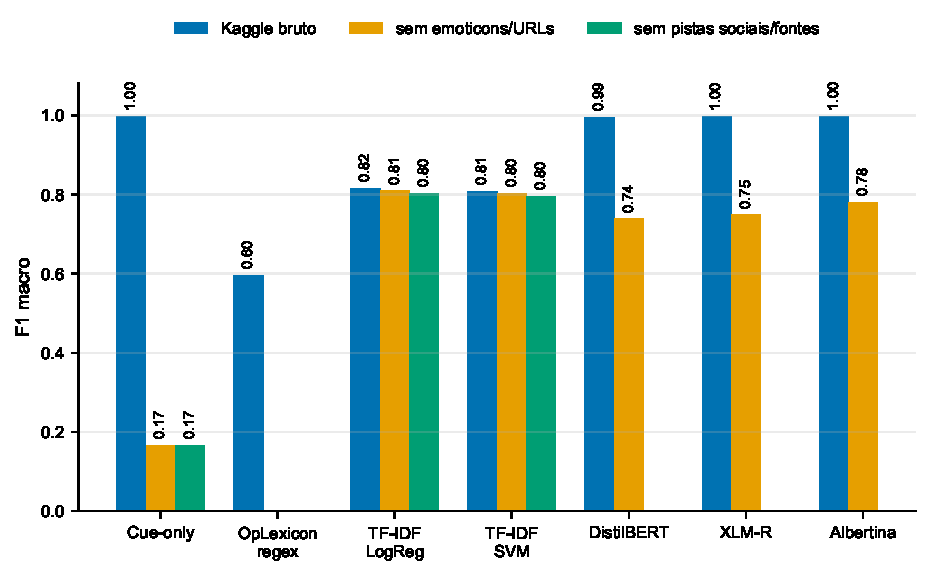
\includegraphics[width=\linewidth]{figures/macro_f1_tracks.pdf}
\caption{F1 macro por sistema e por condição de texto. As barras cinzas hachuradas correspondem ao \emph{split} Kaggle bruto, que tem alta acurácia mas é metodologicamente fraco por conter pistas de rótulo. As barras sem emoticons/URLs e sem pistas sociais/fontes são mais úteis para discutir robustez. Valores ausentes indicam combinações não executadas ou não aplicáveis.}
\label{fig:macro-f1}
\end{figure}

\begin{table}[h]
\small
\centering
\resizebox{\linewidth}{!}{%
\begin{tabular}{@{}lrrrrr@{}}
\toprule
\textbf{Sistema} & \textbf{Treino} & \textbf{Teste} & \textbf{Tratamento} & \textbf{Acurácia} & \textbf{F1 macro} \\
\midrule
OpLexicon com regras & 0 & 4.999 & bruto com pistas & 0,5979 & 0,5960 \\
\textbf{OpLexicon com regras} & \textbf{0} & \textbf{4.999} & \textbf{sem emoticons/URLs} & \textbf{0,3697} & \textbf{0,3668} \\
OpLexicon com regras & 0 & 4.999 & sem pistas sociais/fontes & 0,3695 & 0,3665 \\
TF-IDF + Reg. Logística & 100.000 & 4.999 & bruto com pistas & 0,8172 & 0,8164 \\
\textbf{TF-IDF + Reg. Logística} & \textbf{100.000} & \textbf{4.999} & \textbf{sem emoticons/URLs} & \textbf{0,8086} & \textbf{0,8094} \\
TF-IDF + SVM linear & 100.000 & 4.999 & bruto com pistas & 0,8080 & 0,8084 \\
\textbf{TF-IDF + SVM linear} & \textbf{100.000} & \textbf{4.999} & \textbf{sem emoticons/URLs} & \textbf{0,8020} & \textbf{0,8030} \\
Baseline de pistas & 100.000 & 4.999 & bruto com pistas & 0,9970 & 0,9970 \\
DistilBERT multilíngue & 3.000 & 4.999 & bruto com pistas & 0,9950 & 0,9950 \\
XLM-R base & 3.000 & 4.999 & bruto com pistas & 0,9968 & 0,9968 \\
Albertina 100M pt-BR & 3.000 & 4.999 & bruto com pistas & 0,9972 & 0,9972 \\
\textbf{DistilBERT multilíngue} & \textbf{3.000} & \textbf{4.999} & \textbf{sem emoticons/URLs} & \textbf{0,7465} & \textbf{0,7385} \\
\textbf{XLM-R base} & \textbf{3.000} & \textbf{4.999} & \textbf{sem emoticons/URLs} & \textbf{0,7586} & \textbf{0,7494} \\
\textbf{Albertina 100M pt-BR} & \textbf{3.000} & \textbf{4.999} & \textbf{sem emoticons/URLs} & \textbf{0,7822} & \textbf{0,7808} \\
\bottomrule
\end{tabular}%
}
\caption{Resultados atuais usados como base para a escrita da Etapa 2. As linhas em negrito indicam a condição principal de comparação para cada sistema, sem emoticons e URLs. As linhas ``bruto com pistas'' têm maior acurácia, mas são problemáticas porque a baseline de pistas mostra que o rótulo pode ser inferido quase diretamente por artefatos do corpus. Os resultados neurais são execuções de desenvolvimento com 1.000 exemplos por classe no treino.}
\label{tab:resultados}
\end{table}
\FloatBarrier

\section{Diagnóstico de artefatos e dificuldades encontradas}

A principal dificuldade técnica e metodológica encontrada até aqui foi que o corpus apresenta sinais superficiais fortemente associados aos rótulos. A Figura~\ref{fig:pistas} mostra que 99,28\% dos tweets positivos do teste contêm emoticon positivo, 99,88\% dos negativos contêm emoticon negativo e 99,70\% dos neutros contêm URL. Esse padrão é típico de corpora coletados por supervisão distante, em que emoticons ou outros sinais observáveis são usados para aproximar rótulos de sentimento \citep{go2009distant,wang2015emoticons,yin2021emojification}. O problema não é que esses símbolos sejam irrelevantes em uso real. Emoticons de fato expressam sentimento. O problema é que, neste corpus, eles funcionam quase como a própria etiqueta da classe, tornando a avaliação bruta circular.

Chamamos isso de vazamento de rótulo. O termo descreve a situação em que uma informação muito próxima da resposta aparece na entrada do modelo. Nesse caso, o sistema pode acertar sem resolver a tarefa linguística. O diagnóstico também mostrou que o baseline simbólico não estava imune a esse efeito, pois o OpLexicon contém emoticons polarizados e a execução bruta do sistema simbólico também aproveitava parte desses atalhos.

\begin{figure}[h]
\centering
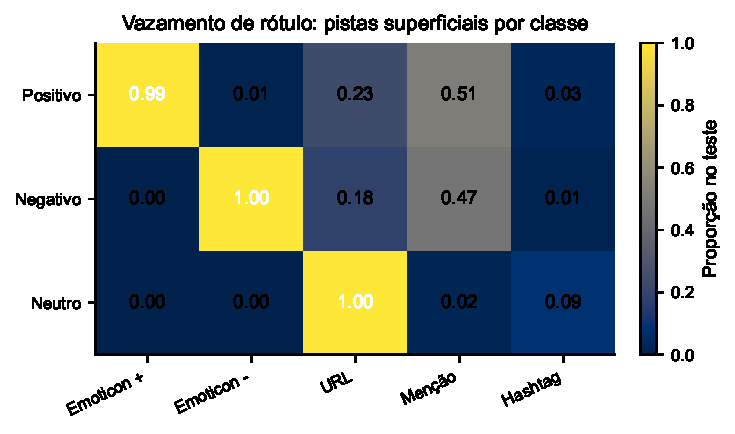
\includegraphics[width=0.82\linewidth]{figures/cue_prevalence_heatmap.pdf}
\caption{Prevalência de pistas superficiais no teste. A concentração quase determinística dessas pistas por classe explica por que uma baseline de pistas alcança desempenho quase perfeito no \emph{split} bruto; portanto, acurácia bruta muito alta deve ser interpretada como alerta, não como vitória automática do modelo.}
\label{fig:pistas}
\end{figure}

Esse achado mudou a interpretação dos resultados. Antes do diagnóstico, os valores quase perfeitos dos transformers pareciam indicar que os modelos tinham aprendido a tarefa. Depois do diagnóstico, a interpretação ficou mais severa. O desempenho bruto quase perfeito é fraco como evidência científica exatamente porque é fácil demais de reproduzir com uma baseline que usa apenas pistas de rótulo. A metodologia adotada segue a lógica de baselines de artefato, em que um classificador propositalmente limitado é usado para medir quanto do dataset pode ser resolvido por pistas indesejadas \citep{gururangan2018artifacts,poliak2018hypothesis}.

\begin{figure}[h]
\centering
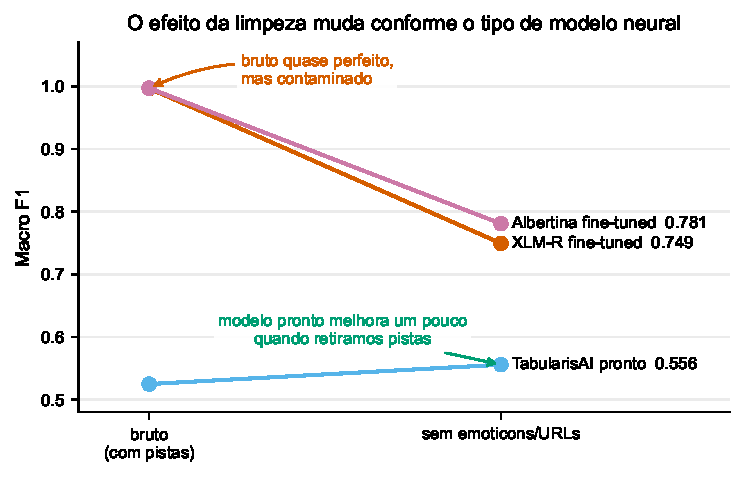
\includegraphics[width=0.72\linewidth]{figures/transformer_drop.pdf}
\caption{Queda de F1 macro dos transformers ao remover emoticons e URLs. O ponto à esquerda é maior, mas não é melhor como evidência metodológica, pois está contaminado por pistas de rótulo. O ponto à direita é menor, porém mais informativo sobre robustez.}
\label{fig:queda-transformers}
\end{figure}

Além da dificuldade metodológica, houve dificuldades práticas. O treino local em MPS no macOS falhou por memória compartilhada em execuções maiores, então as rodadas de desenvolvimento foram feitas em CPU com 1.000 exemplos por classe. Também foi necessário tomar cuidado para que rodadas diferentes não fossem comparadas por engano, já que o mesmo corpus foi testado em versões bruta, limpa e mais estrita. Na aplicação Streamlit, a equipe optou por usar o TF-IDF tratado como opção padrão e manter os transformers no relatório, porque eles exigem mais memória, mais tempo de carregamento e maior cuidado de empacotamento para uma demonstração pública.

\section{Exemplos qualitativos de execução}

Os exemplos qualitativos da Tabela~\ref{tab:exemplos} foram extraídos diretamente das predições salvas. Eles não têm a função de substituir as métricas agregadas, mas ajudam a explicar por que a comparação precisa separar o texto bruto do texto tratado. Em alguns casos, o TF-IDF acerta onde o simbólico falha porque aprende padrões recorrentes do corpus que não aparecem como entradas explícitas do léxico. Em outros, o TF-IDF erra justamente porque o texto limpo fica ambíguo, irônico ou contraditório. O último caso mostra o problema mais importante. O modelo bruto e a baseline de pistas acertam a classe neutra porque a URL funciona como pista quase direta de rótulo, enquanto o conteúdo textual restante parece negativo.

\begin{table}[h]
\small
\centering
\resizebox{\linewidth}{!}{%
\begin{tabularx}{\linewidth}{@{}L{1.1cm}L{2.45cm}Y L{1.9cm} L{2.4cm} Y@{}}
\toprule
\textbf{Índice} & \textbf{Caso} & \textbf{Texto tratado} & \textbf{Esperado} & \textbf{Predições} & \textbf{Leitura} \\
\midrule
2442 & Simbólico falha, TF-IDF acerta & \texttt{poxa ((} & negativo & simbólico indicou neutro; Regressão Logística indicou negativo; SVM linear indicou negativo & O léxico não encontra uma pista polarizada forte depois da remoção do emoticon, enquanto os baselines estatísticos aprendem o padrão recorrente de lamento. \\
1300 & Simbólico falha, TF-IDF acerta & \texttt{É hoje!} & positivo & simbólico indicou neutro; Regressão Logística indicou positivo; SVM linear indicou positivo & O exemplo ilustra uma frase curta sem palavra positiva explícita no OpLexicon, mas frequente em contextos positivos do corpus. \\
2990 & TF-IDF falha em ambiguidade & \texttt{to feliz e com medo ao mesmo tempo} & negativo & Regressão Logística indicou positivo; Albertina indicou negativo; baseline de pistas indicou negativo & A frase mistura \texttt{feliz} e \texttt{medo}. Sem o emoticon negativo original, a Regressão Logística pesa mais a pista positiva e erra. \\
295 & TF-IDF falha em ironia/contradição & \texttt{Tô de boa sim po Encolhida Chorando Nada de demais} & positivo & Regressão Logística indicou negativo; Albertina indicou negativo; baseline de pistas indicou positivo & A frase parece irônica e contém \texttt{Chorando}, mas o rótulo positivo vinha do emoticon original. O caso mostra que a remoção de pistas também revela inconsistências do próprio corpus. \\
3798 & Modelo bruto parece melhor por vazamento & \texttt{Overdose deixou Demi Lovato à beira da morte} & neutro & TF-IDF bruto indicou neutro; baseline de pistas indicou neutro; TF-IDF tratado indicou negativo & No texto original havia uma URL. Como URLs quase sempre marcam a classe neutra no corpus, o acerto bruto não depende de compreender a manchete. \\
\bottomrule
\end{tabularx}%
}
\caption{Casos qualitativos reais extraídos das predições salvas. A baseline de pistas usa apenas a presença de emoticon positivo, emoticon negativo e URL.}
\label{tab:exemplos}
\end{table}
\FloatBarrier

\section{Comparação com a Etapa 1}

O sistema simbólico da Etapa 1 obteve 0,5979 de acurácia e 0,5960 de F1 macro no teste bruto. Após remover emoticons e URLs, o mesmo sistema caiu para 0,3697 de acurácia e 0,3668 de F1 macro. Na versão mais estrita, sem pistas sociais e fontes, ficou em 0,3695 de acurácia e 0,3665 de F1 macro. Portanto, o baseline simbólico bruto também deve ser lido com cuidado. Ele é útil como reprodução da Etapa 1 no corpus original, mas a comparação científica principal com os modelos da Etapa 2 é a condição tratada. Os baselines TF-IDF superam esse valor com margem clara, chegando a 0,8094 de F1 macro sem emoticons e URLs. Esse ganho é esperado, pois os modelos estatísticos aprendem pesos diretamente do corpus e conseguem explorar combinações de palavras que não aparecem como entradas polarizadas no OpLexicon. Além disso, o TF-IDF com Regressão Logística foi escolhido como modelo padrão do Streamlit porque mantém bom desempenho tratado, é leve para deploy e torna a demonstração mais estável.

A comparação com transformers exige duas leituras. No teste bruto, DistilBERT, XLM-R e Albertina ficam próximos de 0,997 de F1 macro, mas esse valor está no mesmo nível da baseline de pistas. Na condição sem emoticons e URLs, Albertina chega a 0,7808 de F1 macro, XLM-R a 0,7494 e DistilBERT a 0,7385. Esses valores continuam acima do sistema simbólico tratado, mas ficam abaixo do TF-IDF tratado. Assim, a conclusão da etapa não é que o transformer bruto ``venceu'' com 99\%, e sim que os transformers são benchmarks úteis para discutir custo computacional, pré-treinamento e robustez, enquanto a comparação principal deve usar a condição limpa.

\section{Limitações e próximos passos}

Os modelos neurais foram treinados em amostras estratificadas de 3.000 exemplos por limitação de tempo e máquina local. Essa decisão deve ser apresentada como limitação experimental, não como falha do fluxo experimental. Os artefatos de desenvolvimento já mostram a queda esperada quando as pistas superficiais são removidas, mas uma execução final maior poderia alterar a ordem relativa entre Albertina, XLM-R e DistilBERT. Outra limitação é que os exemplos qualitativos revelam inconsistências de rotulagem depois da limpeza. Em alguns tweets, o rótulo parece depender mais do emoticon removido do que do texto restante.

Também há uma limitação do corpus. O tratamento sem emoticons/URLs melhora a honestidade da avaliação, mas não remove todos os vieses de coleta. A condição mais estrita, que também remove pistas sociais e marcadores de fontes, mostra que os TF-IDF ainda mantêm F1 macro próximo de 0,80, o que pode indicar tanto aprendizado lexical real quanto novos vieses de tópico. Por isso, essa condição é tratada como diagnóstico adicional, não como uma solução definitiva para o problema de validade externa.

\section{Instruções para execução}

Para preparar o ambiente e rodar os testes, use os comandos abaixo.

\begin{verbatim}
uv sync
uv run pytest
\end{verbatim}

Para reproduzir o baseline simbólico da Etapa 1, use o comando abaixo.

\begin{verbatim}
uv run python \
  etapas/etapa1_simbolica/pipelines/run_symbolic_benchmark_suite.py \
  'text_treatments=[raw,strip_emoticons_urls,strip_social_source_cues]'
\end{verbatim}

Para executar os baselines TF-IDF da Etapa 2, use o comando abaixo.

\begin{verbatim}
uv run python \
  etapas/etapa2_subsimbolica/pipelines/run_classical_benchmark_suite.py
\end{verbatim}

Para executar o diagnóstico de vazamento, use os comandos abaixo.

\begin{verbatim}
uv run python \
  etapas/etapa2_subsimbolica/pipelines/run_leakage_diagnostics.py

uv run python \
  etapas/etapa2_subsimbolica/pipelines/run_leakage_diagnostics.py \
  stripped_treatment=strip_social_source_cues
\end{verbatim}

Para executar um transformer em modo de desenvolvimento, use o comando abaixo.

\begin{verbatim}
uv run --extra transformers python \
  etapas/etapa2_subsimbolica/pipelines/run_transformer_benchmark.py \
  model=xlm_roberta_base train_per_class=1000 \
  model.training.epochs=1 trainer.use_cpu=true
\end{verbatim}

Para abrir a aplicação Streamlit, use o comando abaixo.

\begin{verbatim}
uv run streamlit run streamlit_app.py
\end{verbatim}

A aplicação Streamlit carrega primeiro o modelo TF-IDF tratado versionado para a demonstração. Quando esse modelo está disponível, ele é selecionado como modo padrão. A interface também permite alternar para o leitor simbólico e comparar modelos lado a lado, mas a cópia pública da aplicação evita expor detalhes do corpus, métricas de benchmark e informações internas da avaliação, pois a demonstração final será voltada para uso em feira.

\bibliographystyle{plainnat}
\bibliography{references}

\end{document}
